\pdfminorversion=4
\documentclass[compress,
mathserif,wide,%red,
%handout
]{beamer}

\usepackage{amsmath,amsfonts,bm,bbm,comment}
\usepackage{latexsym,tabularx,amscd}
\usepackage{etex} 
\usepackage{algorithm}
\usepackage[noend]{algorithmic}
\usepackage{subfigure}
\usepackage{url}
%\usepackage{multimedia}
\usepackage{hyperref}
\usepackage{skull}
%\usepackage{enumitem}
%\usepackage{movie15}

\usepackage{multirow}
\usepackage{cancel}

%\usepackage{ulem}
\usepackage{lmodern}
\usepackage{array} 
\usepackage{etoolbox}
\usepackage{caption}
\usepackage[normalem]{ulem}

\usepackage{mathtools}

\usepackage[space]{grffile}

\usepackage{tikz}
\usetikzlibrary{shapes.arrows}
\usetikzlibrary{arrows,positioning}
\usepackage{pgfplots}
%\usetikzlibrary{pgfplots.groupplots}

\tikzset{
    myarrow/.style={
        draw,
        fill=black,
        single arrow,
        minimum height=6ex,
        single arrow head extend=1ex
    }
}


\newcommand{\vertiii}[1]{{\left\vert\kern-0.25ex\left\vert\kern-0.25ex\left\vert #1 
    \right\vert\kern-0.25ex\right\vert\kern-0.25ex\right\vert}}

\newcommand{\vertiiibig}[1]{{\big\vert\kern-0.25ex\big\vert\kern-0.25ex\big\vert #1 
    \big\vert\kern-0.25ex\big\vert\kern-0.25ex\big\vert}}

\newcommand{\vertiiiplain}[1]{{\vert\kern-0.25ex\vert\kern-0.25ex\vert #1 
    \vert\kern-0.25ex\vert\kern-0.25ex\vert}}



\usepackage{dsfont}
\DeclareMathOperator{\ind}{\mathds{1}}  % Indicator


\newcommand{\abs}[1]{\left|#1\right|}

\mode<presentation>

\usetheme{Madrid}
% other themes: AnnArbor, Antibes, Bergen, Berkeley, Berlin, Boadilla,
% boxes, CambridgeUS, Copenhagen, Darmstadt, default, Dresden,
% Frankfurt, Goettingen, Hannover, Ilmenau, JuanLesPins, Luebeck,
% Madrid, Maloe, Marburg, Montpellier, PaloAlto, Pittsburg, Rochester,
% Singapore, Szeged, classic

% \usecolortheme{lily} 
% color themes: albatross, beaver, beetle, crane, default, dolphin,
% dov, fly, lily, orchid, rose, seagull, seahorse, sidebartab,
% structure, whale, wolverine

% \usefonttheme{serif} 
% font themes: default, professionalfonts, serif, structurebold,
% structureitalicserif, structuresmallcapsserif

%\usefonttheme[onlymath]{serif}
%\usefonttheme[onlylarge]{structuresmallcapsserif} 
  
%\useoutertheme[subsection=false]{smoothbars}
% outer themes:
% default,infolines,miniframes,smoothbars,sidebar,split,shadow,tree,smoothtree
%\useinnertheme{rectangles}
\beamertemplatenavigationsymbolsempty

% \definecolor{fore}{RGB}{249,242,215}
% \definecolor{back}{RGB}{51,51,51}
% \definecolor{title}{RGB}{255,0,90}
% \setbeamercolor{titlelike}{fg=title}
% \setbeamercolor{normal text}{fg=fore,bg=back}
% \setbeamercovered{transparent}
  % or whatever (possibly just delete it)
%\beamertemplatenavigationsymbolsempty

\usepackage[english]{babel}
\usepackage[latin1]{inputenc}
% or whatever
%\usepackage{comicsans} 
%\renewcommand{\sfdefault}{comic} 
%\usepackage{mathptmx}
%\mathversion{bold}
%\usepackage{helvet}
%\usepackage{courier}

%\usepackage[T1]{fontenc}
% Or whatever. Note that the encoding and the font should match. If T1
% does not look nice, try deleting the line with the fontenc.


%%%% Figures %%%%%


\newcommand{\LectureFigs}{../Figures}


\definecolor{bluegray}{rgb}{0.15,0.20,0.40}
\definecolor{bluegraylight}{rgb}{0.35,0.40,0.60}
\definecolor{gray}{rgb}{0.3,0.3,0.3}
\definecolor{lightgray}{rgb}{0.7,0.7,0.7}
\definecolor{brightblue}{rgb}{0.1,0.4,0.7}
\definecolor{darkblue}{rgb}{0.1,0.1,0.6}
\definecolor{darkgreen}{rgb}{0.0,0.5,0.2}
\definecolor{orange}{rgb}{0.7,0.3,0}

\def \captioncolor { }

\setbeamertemplate{itemize item}{{\color{black}$\bullet$}}
\setbeamertemplate{itemize subitem}{{\color{black}$\circ$}}
\setbeamertemplate{frametitle}[default][center]
\setbeamerfont{frametitle}{series=\bfseries}
\addtobeamertemplate{frametitle}{\vskip1ex}{ \vspace{0.5em} \hrule}
\setbeamercolor{frametitle}{fg=,bg=}

\setbeamertemplate{theorems}[numbered]
\setbeamertemplate{caption}[numbered]
\setbeamertemplate{algorithm}[numbered]

\numberwithin{theorem}{subsection}
\numberwithin{equation}{subsection}
\numberwithin{figure}{subsection}
\numberwithin{algorithm}{subsection}


%\setbeamerfont{page number in head/foot}{size=\scriptsize}
\setbeamertemplate{footline}[frame number]
\setbeamercolor{page number in head/foot}{fg=black}
\setbeamersize{text margin left=2em,text margin right=2em}

\setbeamertemplate{footline}
{
    %\hspace{3em} \insertshorttitle \hfill \insertframenumber / \inserttotalframenumber\hspace{3em}
    \hspace{3em} \insertshorttitle \hfill \insertsubsectionnumber-\insertframenumber \hspace{3em}
    \vspace{1.5em}
}

\definecolor{babyblueeyes}{rgb}{0.63, 0.79, 0.95}
\definecolor{bleudefrance}{rgb}{0.19, 0.55, 0.91}
\definecolor{matlabPlotBlue}{rgb}{0.25, 0.58, 0.8}
\definecolor{matlabPlotOrange}{rgb}{0.855, 0.324, 0.098}



\captionsetup[figure]{labelfont={color=black}}

\AtBeginEnvironment{lemma}{%
  \setbeamercolor{block title}{fg=black,bg=babyblueeyes}
  \setbeamercolor{block body}{fg=black,bg=}
  \setbeamerfont*{block title}{series=\bfseries}
}

\AtBeginEnvironment{theorem}{%
  \setbeamercolor{block title}{fg=black,bg=babyblueeyes}
  \setbeamercolor{block body}{fg=black,bg=}
  \setbeamerfont*{block title}{series=\bfseries}
}

\AtBeginEnvironment{corollary}{%
  \setbeamercolor{block title}{fg=black,bg=babyblueeyes}
  \setbeamercolor{block body}{fg=black,bg=}
  \setbeamerfont*{block title}{series=\bfseries}
}

\AtBeginEnvironment{fact}{%
  \setbeamercolor{block title}{fg=black,bg=babyblueeyes}
  \setbeamercolor{block body}{fg=black,bg=}
  \setbeamerfont*{block title}{series=\bfseries}
}

\AtBeginEnvironment{definition}{%
  \setbeamercolor{block title}{fg=black,bg=babyblueeyes}
  \setbeamercolor{block body}{fg=black,bg=}
  \setbeamerfont*{block title}{series=\bfseries}
}

\newenvironment<>{varblock}[2][.9\textwidth]{%
  \vspace{-1em}
  \begin{center}
  \begin{minipage}{#1}
  %\setlength{\textwidth}{#1}
  \begin{actionenv}#3%
    \def\insertblocktitle{#2}%
    \par%
    \usebeamertemplate{block begin}}
  {\par%
    \usebeamertemplate{block end}%
  \end{actionenv}
  \end{minipage}
  \end{center}
}


\newcommand\blankfootnote[1]{%
  \let\thefootnote\relax\footnotetext{#1}%
  \let\thefootnote\svthefootnote%
}


%%%%%
\newcommand{\bb}{\bm b}
\newcommand{\bZ}{\bm Z}
\newcommand{\bC}{\bm C}
\newcommand{\cU}{{\cal U}}
\newcommand{\bR}{{\bm R}}
\newcommand{\bi}{{\bm i}}
\newcommand{\bS}{{\bm S}}
\newcommand{\cE}{{\cal E}}
\newcommand{\cF}{{\cal F}}
\newcommand{\bk}{{\bm k}}
\newcommand{\bu}{{\bm u}}
\newcommand{\bx}{{\bm x}}
\newcommand{\bA}{{\bm A}}
\newcommand{\bh}{{\bm h}}
\newcommand{\by}{{\bm y}}
\newcommand{\bI}{{\bm I}}
\newcommand{\ba}{{\bm a}}
\newcommand{\bw}{{\bm w}}
\newcommand{\bPhi}{{\bm \Phi}}
\newcommand{\bX}{{\bm X}}
\newcommand{\bY}{{\bm Y}}
\newcommand{\bM}{{\bm M}}
\newcommand{\be}{{\bm e}}
\newcommand{\bs}{{\bm s}}
\newcommand{\bB}{{\bm B}}
\newcommand{\bW}{{\bm W}}
\newcommand{\bN}{{\bm N}}
\newcommand{\bU}{{\bm U}}
\newcommand{\bV}{{\bm V}}
\newcommand{\bP}{{\bm P}}
\newcommand{\bH}{{\bm H}}
\newcommand{\bSigma}{{\bm \Sigma}}
\newcommand{\bL}{{\bm L}}



\newcommand{\bv}{\bm v}
\newcommand{\eps}{\epsilon}
\newcommand{\vf}{\varphi}
\newcommand{\de}{\delta}
\newcommand{\<}{\langle}
\renewcommand{\>}{\rangle}
\newcommand{\goto}{\rightarrow}
\newcommand{\argmin}{\mbox{argmin}}
\newcommand{\argmax}{\mbox{argmax}}
\newcommand{\Ave}{\mathop{\rm Ave}\nolimits}
\newcommand{\sgn}{\mbox{sgn}}
\newcommand{\cN}{\mathcal{N}}
\newcommand{\cR}{\mathcal{R}}

\def\C{{\mathbb{C}}}
\def\R{{{\mathbb{R}}}} %seemed too large in subscripts, so I changed --JW 
\def\P{{\hbox{\bf P}}}
\def\Z{{{\mathbb{Z}}}}
\def\T{{\hbox{\bf T}}}


\newcommand{\cA}{\mathcal{A}}
\newcommand{\cP}{\mathcal{P}}
\newcommand{\cD}{\mathcal{D}}
\newcommand{\cL}{\mathcal{L}}
\newcommand{\shrink}{\text{shrink}}


\newcommand{\Obs}{\Omega_{\text{obs}}}


\renewcommand{\P}{\operatorname{\mathbb{P}}}
\newcommand{\E}{\operatorname{\mathbb{E}}}

% Linear algebra macros
%\newcommand{\vct}[1]{#1}
%\newcommand{\mtx}[1]{#1}
\newcommand{\vct}[1]{\bm{#1}}
\newcommand{\mtx}[1]{\bm{#1}}
%\newcommand{\mtx}[1]{\mathsfsl{#1}}

\newcommand{\transp}{T}
\newcommand{\adj}{*}
\newcommand{\psinv}{\dagger}
\newcommand{\lspan}[1]{\operatorname{span}{#1}}

\newcommand{\range}{\operatorname{range}}
\newcommand{\colspan}{\operatorname{colspan}}

\newcommand{\rank}{\text{rank}}

\newcommand{\diag}{\operatorname{diag}}
\newcommand{\trace}{\text{Tr}}

\newcommand{\supp}[1]{\operatorname{supp}(#1)}

\newcommand{\smax}{\sigma_{\max}}
\newcommand{\smin}{\sigma_{\min}}

\newcommand{\restrict}[1]{\big\vert_{#1}}

\newcommand{\Id}{\text{\em I}}
\newcommand{\OpId}{\mathcal{I}}



% define your own colors:
\definecolor{Red}{rgb}{1,0,0}
\definecolor{Blue}{rgb}{0,0,1}
\definecolor{Green}{rgb}{0,1,0}
\definecolor{magenta}{rgb}{1,0,.6}
\definecolor{lightblue}{rgb}{0,.5,1}
\definecolor{lightpurple}{rgb}{.6,.4,1}
\definecolor{gold}{rgb}{.6,.5,0}
\definecolor{orange}{rgb}{1,0.4,0}
\definecolor{hotpink}{rgb}{1,0,0.5}
\definecolor{newcolor2}{rgb}{.5,.3,.5}
\definecolor{newcolor}{rgb}{0,.3,1}
\definecolor{newcolor3}{rgb}{1,0,.35}
\definecolor{darkgreen1}{rgb}{0, .35, 0}
\definecolor{darkgreen}{rgb}{0, .6, 0}
\definecolor{darkred}{rgb}{.75,0,0}

\xdefinecolor{olive}{cmyk}{0.64,0,0.95,0.4}
\xdefinecolor{purpleish}{cmyk}{0.75,0.75,0,0}

\definecolor{lightgrey}{RGB}{186,186,186}
\definecolor{back}{RGB}{51,51,51}
\definecolor{fore}{RGB}{249,242,215}
\definecolor{back}{RGB}{51,51,51}
\definecolor{title}{RGB}{255,0,20}
\definecolor{keywords}{RGB}{255,0,90}
\definecolor{comments}{RGB}{60,179,113}
\definecolor{cobalt}{RGB}{102,153,204}

\def \itemstyle {\bf}
\def \itemhighlight {\bf}  

% \definecolor{blockbodycolor}{RGB}{30,30,40}
% \definecolor{blocktitlecolor}{RGB}{55,55,75}
\definecolor{blockbodycolor}{RGB}{186,206,232}
\definecolor{blocktitlecolor}{RGB}{55,55,75}

\setbeamercolor{titlelike}{fg=darkred,bg=white}
\setbeamercolor{normal text}{fg=black,bg=white}
\setbeamercolor{block title}{fg=white,bg=blocktitlecolor}
\setbeamercolor{block body}{bg=blockbodycolor}
\setbeamercolor{alerted text}{fg=darkred}
\setbeamercolor{title}{fg=darkred,bg=lightgrey}


\newcommand{\alertb}[1]{\textcolor{blue}{ #1}}

\newcommand{\yp}[1]{\textcolor{red}{ #1}}
\newcommand{\zeronorm}[1]{\left\|#1 \right\|_0}
\newcommand{\unorm}[1]{\left\|#1 \right\|_u}
\newcommand{\ynorm}[1]{\left\|#1 \right\|_{\bar{y}}}
\newcommand{\onetwonorm}[1]{\left\|#1\right\|_{1,2}}
\newcommand{\opnorm}[1]{\left\|#1\right\|}
\newcommand{\fronorm}[1]{\left\|#1\right\|_{F}}
\newcommand{\onenorm}[1]{\left\|#1\right\|_{\ell_1}}
\newcommand{\twonorm}[1]{\left\|#1\right\|_{2}}
\newcommand{\oneinfnorm}[1]{\left\|#1\right\|_{1,\infty}}
\newcommand{\infnorm}[1]{\left\|#1\right\|_{\ell_\infty}}
\newcommand{\nucnorm}[1]{\left\|#1\right\|_*}

%\makeatletter
%\def\th@mystyle{%
%    \normalfont % body font
%    \setbeamercolor{block title example}{bg=,fg=black}
%    \setbeamerfont{block title example}{series=\bfseries}
%    \setbeamercolor{block body example}{bg=,fg=black}
%    %\setbeamertemplate{exampleblock}[numbered]
%    \def\inserttheoremblockenv{exampleblock}
%  }
%\makeatother
%\theoremstyle{mystyle}
%\newtheorem*{lem}{Lemma}

\setbeamertemplate{frametitle continuation}{}


\newcommand{\courseTitle}{STAT 37797: Mathematics of Data Science} 



% \subtitle
% {Include Only If Paper Has a Subtitle}

\vspace{.5cm}

\author{Yuxin Chen}

\institute[Princeton] % (optional, but mostly needed)
{Princeton University}


% - Use the \inst command only if there are several affiliations.
% - Keep it simple, no one is interested in your street address.


\subject{Beamer}
% This is only inserted into the PDF information catalog. Can be left
% out.

% Delete this, if you do not want the table of contents to pop up at
% the beginning of each subsection:
% \AtBeginSubsection[]
% {
%   \begin{frame}<beamer>
%     \frametitle{Outline}
%     \tableofcontents[currentsection,currentsubsection]
%   \end{frame}
% }






\graphicspath{{../../../Figures/}}


\title % (optional, use only with long paper titles)
{Refined analysis of local convergence: implicit regularization}

\defbeamertemplate*{title page}{customized}[1][]
{

  \hfill {\em \courseTitle}

  \begin{center}
    \vspace{2.5em}
    \usebeamerfont{title} {\Large\bf\inserttitle} \par
  
    \vspace{1.5em}
    \includegraphics[width=2cm]{\LectureFigs/UC_logo.png} 
  
    \vspace{1em}
    {\large Cong Ma \par }

    \vspace{0.2em}
    { \large \quad University of Chicago, Autumn 2021 }
  \end{center}

  \vfill
}

\setcounter{subsection}{9}

\begin{document}

\begin{frame}[plain]
  \titlepage

\end{frame}








\begin{frame}
\frametitle{A natural least-squares formulation}

\begin{eqnarray*}
	\text{given:}\qquad y_k &= &(\vct{a}_k^\top\vct{x}^{\star})^2, \quad  1\leq k \leq m  
\end{eqnarray*}

\vspace{-2em}
\begin{align*}
	\Downarrow
\end{align*}
\vspace{-2em}
%
%One may attempt recovery by solving
%
\begin{align*} 
	%\label{eq:least-squares-PR}
	\text{minimize}_{\bm{x}\in \mathbb{R}^n}\quad f(\bm{x})=\frac{1}{4m}\sum_{k=1}^{m}\Big[ \big(\bm{a}_{k}^{\top}\bm{x}\big)^{2}-y_{k} \Big]^{2}
\end{align*}
%
\bigskip

\begin{itemize}
	\itemsep1em
	\pause
	\item {\bf pros:} often exact as long as sample size is sufficiently large
	\pause
	\item {\bf cons:} $f(\cdot)$ is highly nonconvex \\
		\hspace{6em} $\longrightarrow$~ {\em computationally challenging!} 
\end{itemize}

\end{frame}




\begin{frame}
\frametitle{Wirtinger flow (Cand\`es, Li, Soltanolkotabi\,'14)}

\[
\text{minimize}_{\bm{x}}\quad f(\bm{x})=\frac{1}{4m}\sum_{k=1}^{m}\Big[ \big(\bm{a}_{k}^{\top}\bm{x}\big)^{2}-y_{k} \Big]^{2}
\]


\pause

\vspace{-2em}


\begin{columns}
\begin{column}{0.3\textwidth}

\begin{center}
  \includegraphics[width=1.05\textwidth,angle=-40]{GD2.png}
\end{center}

\end{column}



\begin{column}{0.7\textwidth}

\begin{itemize}
\itemsep1em
\item {\bf spectral initialization:}  $\bm{x}^{0}~\leftarrow~$ leading eigenvector of certain data matrix
	%\[
	%\frac{1}{m}\sum_{i=1}^{m}(\bm{a}_{i}^{\top}\bm{x}^{\star})^{2}\bm{a}_{i}\bm{a}_{i}^{\top}
	%\]
\pause
\item {\bf gradient descent:}  
\[
  \vct{x}^{t+1}= \vct{x}^t- \eta \, \nabla f(\vct{x}^t), \qquad t=0,1,\cdots
\]
\end{itemize}

\end{column}
\end{columns}

\end{frame}


\begin{frame}
	\frametitle{First theory of WF}

	

 
\hfill $\mathsf{dist}(\vct{x}^t, \vct{x}^{\star}) := \min \{ \|\vct{x}^t \pm \vct{x}^{\star} \|_2 \}$


\begin{theorem}[Cand\`es, Li, Soltanolkotabi\,'14]
Under i.i.d.~Gaussian design, WF with spectral initialization achieves
\[
	\mathsf{dist}(\vct{x}^t, \vct{x}^{\star}) \lesssim \left( 1 - \frac{\eta}{4} \right)^{t/2} \|\vct{x}^{\star} \|_2, 
\]
%
with high prob., 
	provided that step size $\only<2>{\alert{\eta \lesssim 1/n}}\only<1,3>{\eta \lesssim 1/n}$ and
	sample size: $ \only<3>{\alert{m\,\gtrsim\, n\log n}}\only<1,2>{\alert{m\,\gtrsim\, n\log n}} $.
\end{theorem}
%

%
\begin{itemize}
  \itemsep0.5em
  \item<2-> Iteration complexity:  $O\big(n \log\frac{1}{\epsilon}\big)$  
  \item<3-> Sample complexity: $O(n\log n)$
  \item<4-> Derived based on (worst-case) local geometry 
\end{itemize}

\end{frame}
\begin{frame}
	\frametitle{What does optimization theory say about WF?}
	

\vspace{-3em}

	\begin{center}
	\begin{equation*}
		\textit{Gaussian designs: } \bm{a}_k ~ \overset{\mathrm{i.i.d.}}{\sim}~ \mathcal{N}(\bm{0}, \bm{I}_n), \quad 1\leq k \leq m
	\end{equation*}
	\end{center}

	\vfill

%\begin{comment}
%\end{comment}

\uncover<2->{

%\vspace{-11em}

	{\bf Finite-sample level ($m\asymp n\log n$) } 
	\[
 		\nabla^2 f(\bm{x}) ~\succ \bm{0} \quad  
		\uncover<3->{ \underset{ {\alert{\text{condition number}~\asymp~ n}} }{\underbrace{ \text{but ill-conditioned } }}  ~\text{(even locally)} }
	\]

	\vfill	

\uncover<4->
{
\setbeamercolor{block body}{bg=babyblueeyes,fg=black}

\begin{varblock}[\textwidth]{}
\begin{center}
  	{\bf Consequence (Cand\`es et al '14)}:\quad WF attains $\varepsilon$-accuracy within \\ \alert{$O\big(n\log\frac{1}{\varepsilon}\big)$} iterations if $m \asymp n \log n$
\end{center}
\end{varblock}
}
}

\end{frame}




\begin{frame}
	\frametitle{Generic optimization theory gives pessimistic bounds}

\begin{columns}

\begin{column}{0.92\textwidth}
\begin{itemize}
  \item[] WF converges in $O(n)$ iterations
  \pause

  \vspace{-1em}
  \begin{figure}
	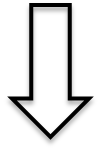
\includegraphics[width=0.05\textwidth,angle=180]{arrow_down_3.png} \qquad 
  \end{figure}

  \item[] Step size taken to be \alert{$\eta = O(1/n)$}

  \pause
  \vspace{-1em}
  \begin{figure}
	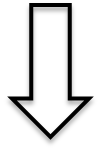
\includegraphics[width=0.05\textwidth,angle=180]{arrow_down_3.png} \qquad 
  \end{figure}


  \item[] This choice is suggested by \only<3->{\alert{worst-case}} optimization theory

  
  \uncover<4->{
  \vspace{-1em}
  \begin{figure}
	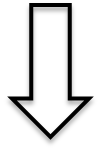
\includegraphics[width=0.05\textwidth,angle=180]{arrow_down_3.png}
  \end{figure}


  \item[] Does it capture what really happens? 

  }
\end{itemize}

\end{column}
\end{columns}

\end{frame}


\begin{frame}
	\frametitle{Improved theory of WF}


\hfill $\mathsf{dist}(\vct{x}^t, \vct{x}^{\star}) := \min \{ \| \vct{x}^t \pm \vct{x}^{\star} \|_2 \}$


\begin{theorem}[Ma, Wang, Chi, Chen\,'17]
Under i.i.d.~Gaussian design, WF with spectral initialization achieves 
	$$ \mathsf{dist}( \bm{x}^{t}, \bm{x}^\star ) \lesssim \left(1-\frac{\eta}{2}\right)^{t} \|\bm{x}^\star\|_{2}$$
with high prob., 
provided that step size $\alert{\eta \asymp 1 / \log n}$ and
$ \text{sample size}~ m \gtrsim n \log n $.
\end{theorem}


\begin{itemize}
  \itemsep0.5em
  \item Iteration complexity:  $O\big(n \log\frac{1}{\epsilon}\big)$   $\searrow$~~  \alert{$O\big( \log n \log\frac{1}{\epsilon} \big)$}
  \item Sample complexity: $O(n\log n)$
  \item Derived based on finer analysis of GD trajectory
\end{itemize}

\end{frame}







\begin{frame}
	\frametitle{What does optimization theory say about WF?}
	

\vspace{-3em}

	\begin{center}
	\begin{equation*}
		\textit{Gaussian designs: } \bm{a}_k ~ \overset{\mathrm{i.i.d.}}{\sim}~ \mathcal{N}(\bm{0}, \bm{I}_n), \quad 1\leq k \leq m
	\end{equation*}
	\end{center}

	\vfill

%\begin{comment}
%\end{comment}

\uncover<2->{

%\vspace{-11em}

	{\bf Finite-sample level ($m\asymp n\log n$) } 
	\[
 		\nabla^2 f(\bm{x}) ~\succ \bm{0} \quad  
		\uncover<3->{ \underset{ {\alert{\text{condition number}~\asymp~ n}} }{\underbrace{ \text{but ill-conditioned } }}  ~\text{(even locally)} }
	\]

	\vfill	

\uncover<4->
{
\setbeamercolor{block body}{bg=babyblueeyes,fg=black}

\begin{varblock}[\textwidth]{}
\begin{center}
  	{\bf Consequence (Cand\`es et al '14)}:\quad WF attains $\varepsilon$-accuracy within \\ \alert{$O\big(n\log\frac{1}{\varepsilon}\big)$} iterations if $m \asymp n \log n$
\end{center}
\end{varblock}
}
}

\end{frame}




\begin{frame}
	\frametitle{Generic optimization theory gives pessimistic bounds}

\begin{columns}

\begin{column}{0.92\textwidth}
\begin{itemize}
  \item[] WF converges in $O(n)$ iterations
  \pause

  \vspace{-1em}
  \begin{figure}
	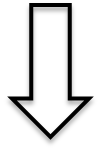
\includegraphics[width=0.05\textwidth,angle=180]{arrow_down_3.png} \qquad 
  \end{figure}

  \item[] Step size taken to be \alert{$\eta = O(1/n)$}

  \pause
  \vspace{-1em}
  \begin{figure}
	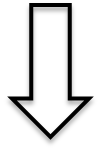
\includegraphics[width=0.05\textwidth,angle=180]{arrow_down_3.png} \qquad 
  \end{figure}


  \item[] This choice is suggested by \only<3->{\alert{worst-case}} optimization theory

  
  \uncover<4->{
  \vspace{-1em}
  \begin{figure}
	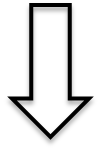
\includegraphics[width=0.05\textwidth,angle=180]{arrow_down_3.png}
  \end{figure}


  \item[] Does it capture what really happens? 

  }
\end{itemize}

\end{column}
\end{columns}

\end{frame}




\begin{frame}
	\frametitle{Numerical efficiency with $\eta_t  = 0.1$}
\begin{figure}
	\centering
	\includegraphics[width=0.7\textwidth]{pr_const_stepsize.pdf}
\end{figure}

{
\setbeamercolor{block body}{bg=babyblueeyes,fg=black}

\begin{varblock}[\textwidth]{}
\begin{center}
  	Vanilla GD (WF) converges fast for a constant step size! 
\end{center}
\end{varblock}
}


\end{frame}



\begin{frame}
	\frametitle{A second look at gradient descent theory}

\vspace{-0.2em}
Which local region enjoys both strong convexity and smoothness? 

\bigskip
\bigskip

\uncover<1,2>{
\[
	\nabla^2 f(\bm{x})= \frac{1}{m}\sum_{k=1}^m \left[ \alert{3\big(\bm{a}_k^\top \bm{x}\big)^2} -\big(\bm{a}_{k}^{\top}\bm{x}^\star\big)^2\right]\bm{a}_k\bm{a}_k^\top
\]

}

\bigskip

\uncover<2>{
\begin{itemize}
  \item Not sufficiently smooth if $\bm{x}$ and $\bm{a}_k$ are too close (coherent)
\end{itemize}
}

\uncover<3->{

\vspace{-8.6em}

\begin{figure}
	\only<1,2>{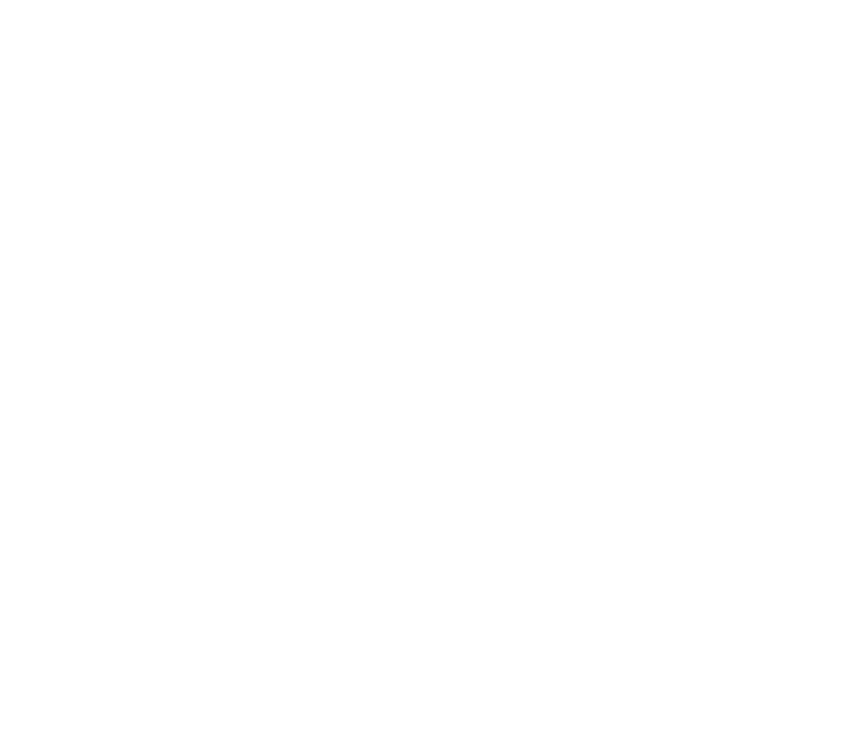
\includegraphics[width=0.6\textwidth]{WF_region_0.pdf}}\only<3>{\includegraphics[width=0.6\textwidth]{WF_region_2.pdf}}\only<4->{\includegraphics[width=0.6\textwidth]{WF_region_1.pdf}}
\end{figure}

\vspace{-2.5em}

\begin{itemize}
  \itemsep0.5em
  %\item<3-> $\bm{x}$ is not far away from $\bm{x}^{\star}$
  \item<2-> $\bm{x}$ is incoherent w.r.t.~sampling vectors $\{\bm{a}_k\}$ \alert{(incoherence region)}
\end{itemize}
}

\uncover<5->{
{
\setbeamercolor{block body}{bg=babyblueeyes,fg=black}

\begin{varblock}[\textwidth]{}
\begin{center}
	Prior works suggest enforcing \alert{regularization} (e.g.~truncation, projection, regularized loss) to promote incoherence
\end{center}
\end{varblock}
}
}




\end{frame}



\begin{comment}
\begin{frame}
	\frametitle{A second look at gradient descent theory}


\begin{center}
	\begin{tabular}{cc}
 	 	
\includegraphics[width=0.04\textwidth]{\ProbFigs/shade.png} 	&  region of local strong convexity + smoothness \tabularnewline
	\end{tabular} 
\end{center}

\vspace{-1em}

\begin{columns}

\begin{column}{0.38\textwidth}
\begin{figure}
	\only<1>{\includegraphics[width=0.9\textwidth]{\ProbFigs/circle0.png}}\only<2>{\includegraphics[width=0.9\textwidth]{\ProbFigs/circle1.png}}\only<3>{\includegraphics[width=0.9\textwidth]{\ProbFigs/circle2.png}}\only<4->{\includegraphics[width=0.9\textwidth]{\ProbFigs/circle3.png}}
\end{figure}
\end{column}

\begin{column}{0.42\textwidth}
\begin{figure}
	\only<1-4>{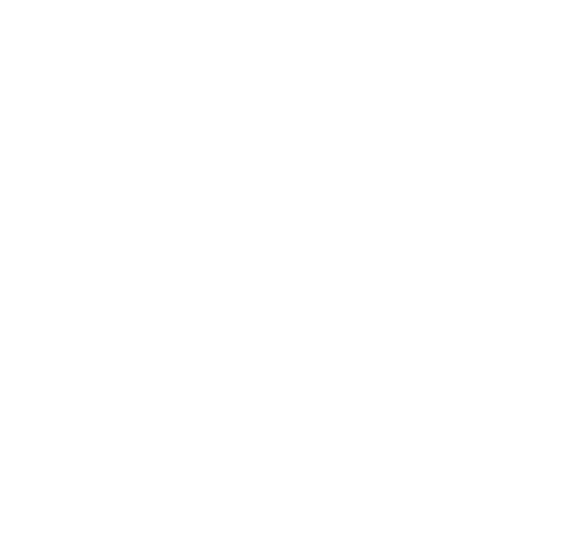
\includegraphics[width=\textwidth]{\ProbFigs/GD_WF_ball5.pdf}}\only<5>{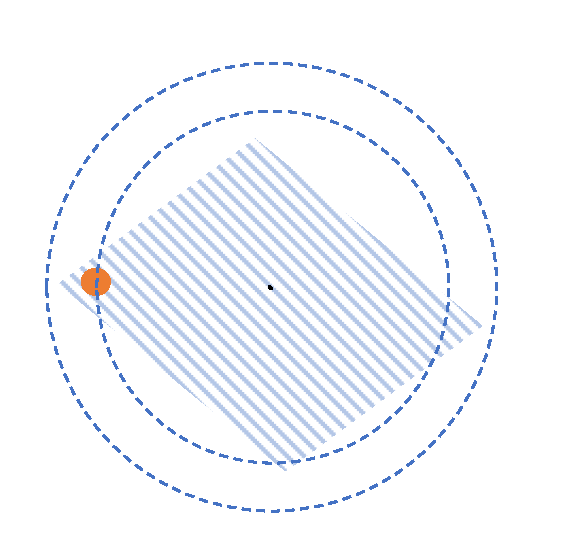
\includegraphics[width=\textwidth]{\ProbFigs/GD_WF_ball4.pdf}}\only<6>{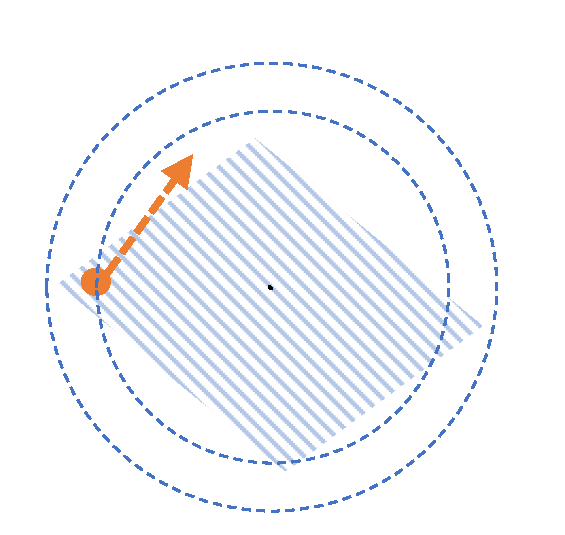
\includegraphics[width=\textwidth]{\ProbFigs/GD_WF_ball3.pdf}}\only<7>{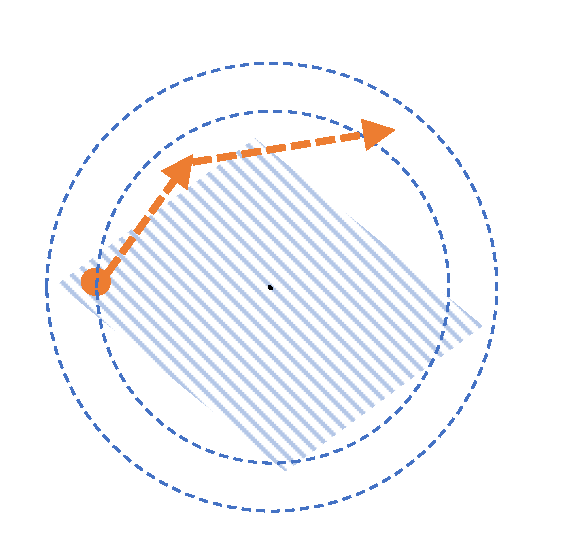
\includegraphics[width=\textwidth]{\ProbFigs/GD_WF_ball2.pdf}}\only<8->{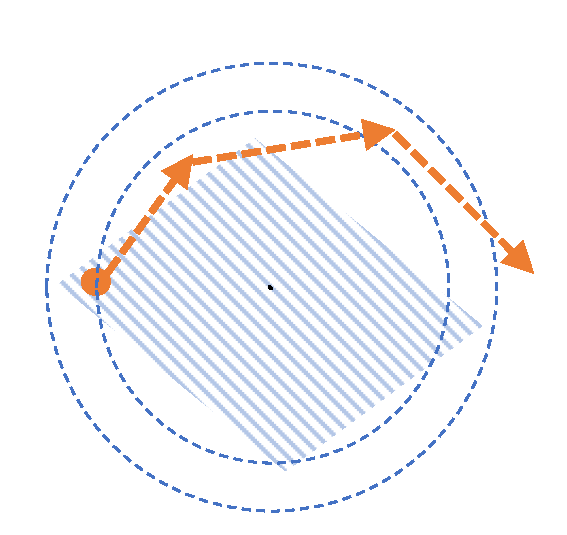
\includegraphics[width=\textwidth]{\ProbFigs/GD_WF_ball1.pdf}}
\end{figure}
\end{column}

\end{columns}
\vfill
\begin{itemize}
  \itemsep0.5em
  \item  Generic optimization theory only ensures that iterates  remain in $\ell_2$ ball but not incoherence region
%  \item<9-> {\em Prior theory enforces regularization to promote incoherence}
\end{itemize}


\end{frame}
\end{comment}






\begin{frame}
	\frametitle{Encouraging message: GD is implicitly regularized}


\begin{center}
	\begin{tabular}{cc}
 	 	
\includegraphics[width=0.04\textwidth]{shade.png} 	&  region of local strong convexity + smoothness \tabularnewline
	\end{tabular} 
\end{center}

\vspace{-3em}

\begin{columns}


\begin{column}{0.42\textwidth}
\begin{figure}
	\only<1>{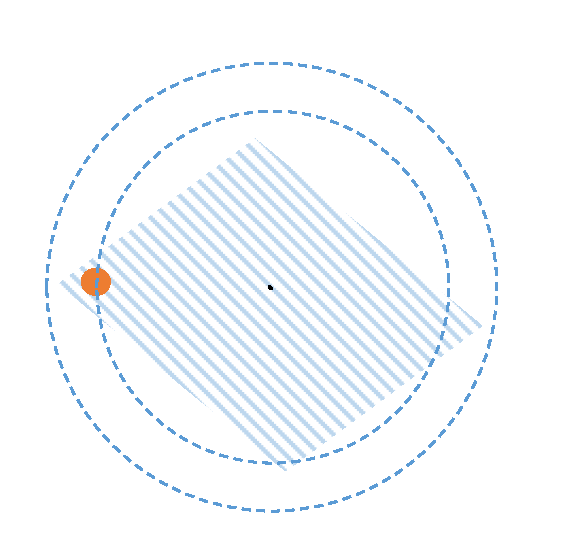
\includegraphics[width=\textwidth]{GD_WF_ball4_good.pdf}}\only<2>{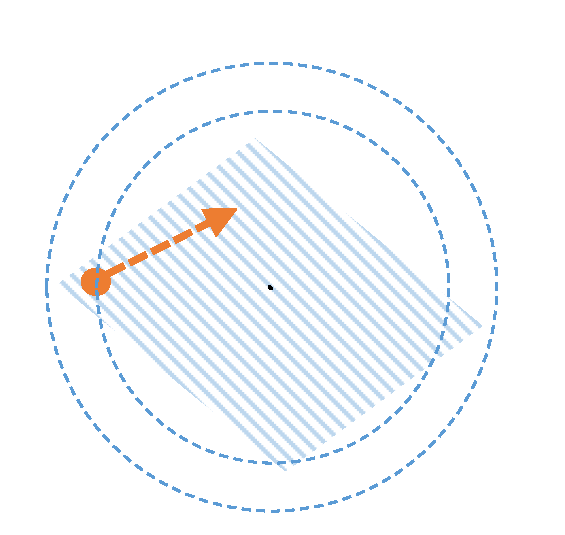
\includegraphics[width=\textwidth]{GD_WF_ball3_good.pdf}}\only<3>{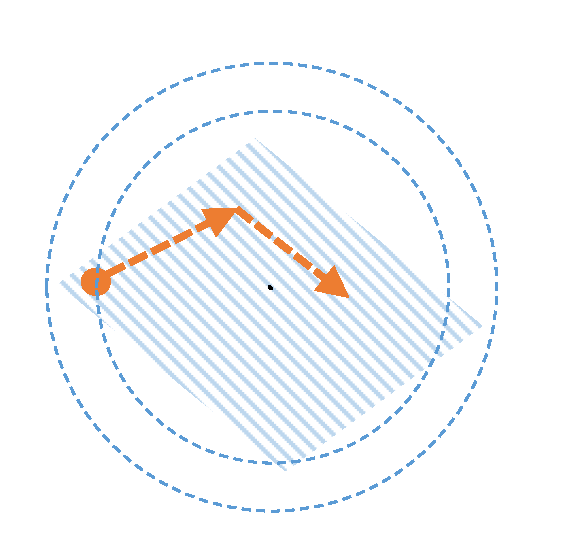
\includegraphics[width=\textwidth]{GD_WF_ball2_good.pdf}}\only<4->{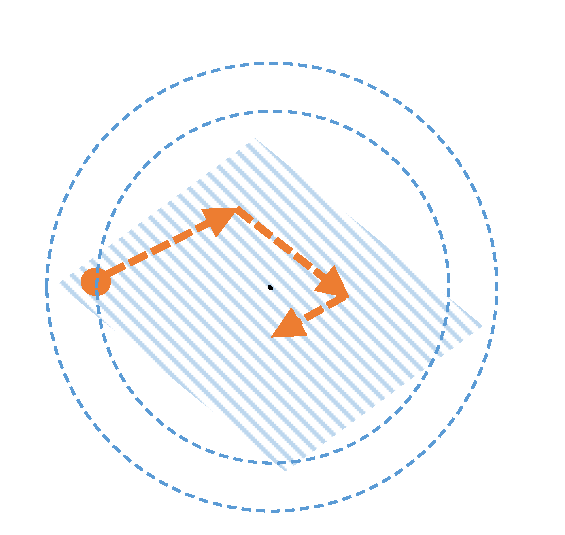
\includegraphics[width=\textwidth]{GD_WF_ball1_good.pdf}}
\end{figure}

\end{column}

\end{columns}
\vfill


\uncover<5->{
{
\setbeamercolor{block body}{bg=babyblueeyes,fg=black}

\begin{varblock}[0.9 \textwidth]{}
\begin{center}
	GD implicitly forces iterates to remain  \alert{incoherent with $\{\bm{a}_k\}$} 
$\max_k \big| \bm{a}_k^{\top} (\bm{x}^{t}- \bm{x}^{\star} ) \big | \lesssim \sqrt{\log n} \, \| \bm{x}^{\star} \|_2,\quad \forall t$
\end{center}
\end{varblock}
}

\pause
	\begin{itemize}
		\item[{\color{black}---}] cannot be derived from generic optimization theory;  relies on finer statistical analysis for entire trajectory of GD 
	\end{itemize}

}


\end{frame}


\begin{frame}
	\frametitle{Theoretical guarantees for local refinement stage}



\begin{theorem}[Ma, Wang, Chi, Chen\,'17]
Under i.i.d.~Gaussian design, WF with spectral initialization achieves 
\begin{itemize}
	\itemsep0.3em
	\item $  \max_k \big| \bm{a}_k^{\top} \bm{x}^{t}  \big | \lesssim \sqrt{\log n} \, \| \bm{x}^{\star} \|_2$ ~(incoherence)
	\pause
	\item 
		$\mathsf{dist}(\bm{x}^{t}, \bm{x}^\star) \lesssim \left(1-\frac{\eta}{2}\right)^{t} \|\bm{x}^\star\|_{2}$ ~(linear convergence)
\end{itemize}
provided that step size $\alert{\eta \asymp 1/ \log n}$ and
$ \text{sample size}~ m \gtrsim n\log n $.
\end{theorem}



\vfill

\begin{itemize}
	\itemsep0.5em
	\item Attains $\varepsilon$ accuracy within $O\big(\log n \,\log \frac{1}{\varepsilon}\big)$ iterations
\end{itemize}

\end{frame}





\begin{frame}
	\frametitle{Key proof idea: leave-one-out analysis}
For each $1\leq l\leq m$, introduce leave-one-out iterates $\bm{x}^{t,(l)}$ \\ by dropping $l$th measurement
\vfill
\uncover<1->{

\begin{figure}
\centering
\includegraphics[width=0.85\textwidth]{pr_leave_one_out.pdf}
\end{figure}
}

\end{frame}



\begin{frame}
	\frametitle{Key proof idea: leave-one-out analysis}

\begin{figure}
\centering
 \only<1>{\includegraphics[width=0.45\textwidth]{LOO_sequence.pdf}}\only<2->{\includegraphics[width=0.45\textwidth]{LOO_original_sequence.pdf}}
\end{figure}
\begin{itemize}
	\itemsep0.5em
	\item Leave-one-out iterate $\bm{x}^{t,(l)}$ is independent of $\bm{a}_l$
		%, and are hence {\bf incoherent} w.r.t.~$\bm{a}_l$ with high prob.
	\item<2-> Leave-one-out iterate $\bm{x}^{t,(l)}$ ~$\approx$~ true iterate $\bm{x}^{t}$ 
	\item<3->[] \qquad\qquad $\Longrightarrow~~\bm{x}^{t}$ is $\underset{\alertb{\text{nearly orthogonal to}}}{\underbrace{\text{nearly independent of}}}$  $\bm{a}_{l}$
\end{itemize}
\end{frame}




\begin{comment}

\begin{frame}
	\frametitle{Incoherence region in high dimensions}

\begin{center}
\begin{tabular}{cc}
 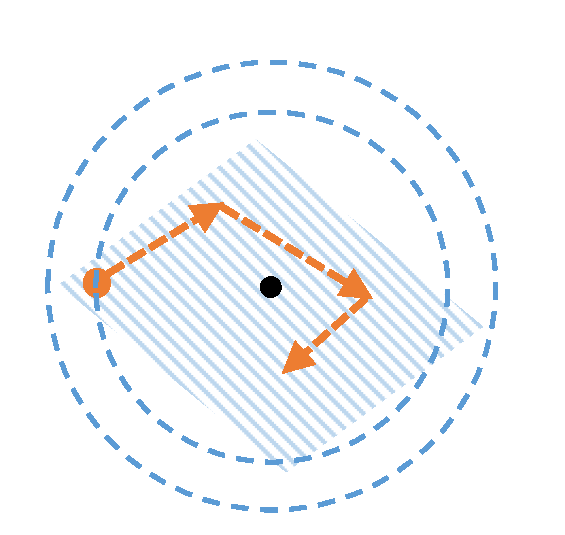
\includegraphics[width=0.4\textwidth]{\yuxinRegFigs/GD_converge_2D.pdf}& 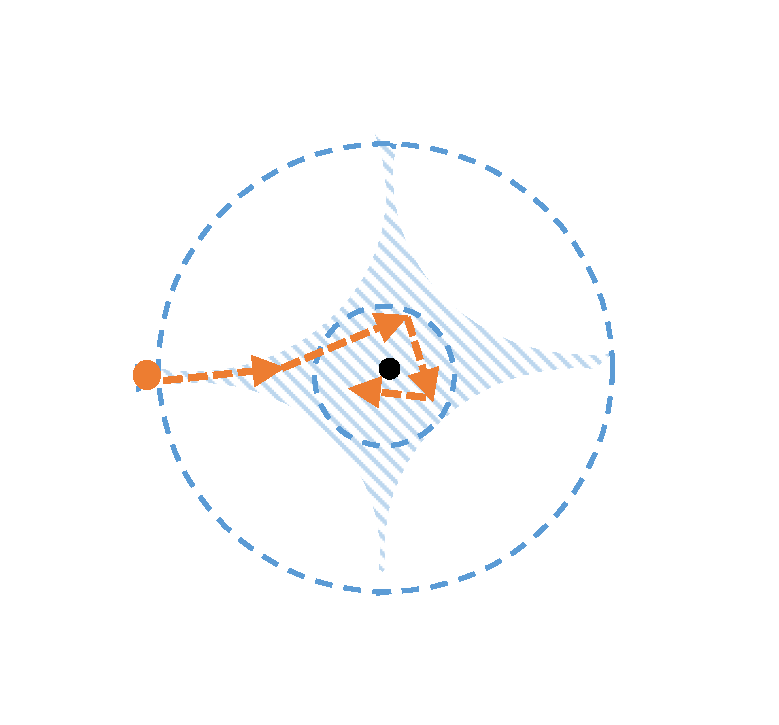
\includegraphics[width=0.4\textwidth]{\yuxinRegFigs/GD_converge_highD.pdf}\tabularnewline
 2-dimensional & $\underset{\alertb{\text{incoherence region is vanishingly small}}}{\underbrace{\text{high-dimensional (mental representation)}}}$ \tabularnewline
\end{tabular}
%
\end{center}
\end{frame}

\end{comment}






\begin{frame}
\frametitle{No need of sample splitting}

\begin{itemize}
  \item Several prior works use sample-splitting: require \alert{fresh samples} at each iteration; not practical but helps analysis 
\end{itemize}
  \begin{center}
     \includegraphics[width=0.65\textwidth]{path_fresh.pdf} 
  \end{center}


\uncover<2>{
\begin{itemize}
     \item  {\bf This tutorial:} reuses all samples in all iterations
\end{itemize}
  \begin{center}
     \includegraphics[width=0.65\textwidth]{path_dependent.pdf} 
  \end{center}
}

\end{frame}




\begin{frame}[plain]

\vfill
\begin{center}
  {\Large \bf Low-rank matrix completion}
\end{center}
\vfill

\end{frame}

%\begin{frame}
%	\frametitle{XXX}
%	only present the result using regularity condition, and mention that projection is not needed
%\end{frame}

\end{document}

